\documentclass{article}

\usepackage{listings} % For source code
\usepackage{enumerate}
\usepackage{graphicx} % For images
\usepackage{float}    % For tables and other floats
\usepackage{subfig}   % For subfigures
\usepackage{epstopdf}

\usepackage[usenames,dvipsnames]{color}


\definecolor{mygrey}{gray}{.96} % Light Grey
\definecolor{BrickRed}{RGB}{120,0,0}
\lstset{
	language=C++,              % choose the language of the code ("language=Verilog" is popular as well)
   tabsize=3,							  % sets the size of the tabs in spaces (1 Tab is replaced with 3 spaces)
	basicstyle=\footnotesize,               % the size of the fonts that are used for the code
	numbers=left,                   % where to put the line-numbers
	numberstyle=\footnotesize,              % the size of the fonts that are used for the line-numbers
	stepnumber=1,                   % the step between two line-numbers. If it's 1 each line will be numbered
	numbersep=5pt,                  % how far the line-numbers are from the code
	backgroundcolor=\color{mygrey}, % choose the background color. You must add \usepackage{color}
	showspaces=false,              % show spaces adding particular underscores
	showstringspaces=false,        % underline spaces within strings
	showtabs=false,                % show tabs within strings adding particular underscores
	frame=single,	                 % adds a frame around the code
	tabsize=3,	                    % sets default tabsize to 2 spaces
	captionpos=b,                   % sets the caption-position to bottom
	breaklines=true,                % sets automatic line breaking
	breakatwhitespace=false,        % sets if automatic breaks should only happen at whitespace
	%escapeinside={\%*}{*)},        % if you want to add a comment within your code
	commentstyle=\color{BrickRed}   % sets the comment style
}


\title{\LARGE MA 226 : Monte Carlo Simulation\\ \textbf{Project}}
\author{\large KadambalaAnil\\ \textbf{140123016}\\\\Shalu Rungta(140123033)\\Sandeep Kumar(14012330)\\Priya Meena(140123025)\\Korrapati Harsha Vardhan(140123019)}
\date{13/04/2016}
\begin{document}
\maketitle
\textbf{Q1.}\\\\
Given $F(x)=(1+\lambda)F_{1}(x)-\lambda F_{1}^2(x)$.\\\\Generate random numbers following the disribution $F(x)$.Here, $F_{1}(x)$ is the CDF of normal distribution.\\\\a.)Use Inverse-Transformation Method\\\\b.)Use Acceptance-Rejectance Method\\\\\\
\textbf{Q1(a)}\\\\
Suppose we want to generate a random variable $X$ with the property that $P(X<=x)=F(x)$  $\forall x$. The inverse transform method sets : $X=F^{-1}(U)$, $U \sim U(0,1)$, where $U(0,1)$ is a uniform distribution on $[0,1]$.\\\\So, substituting $F(x)=U $ and assuming $F_{1}(x)=u_1$, we get a quadratic equation in $u_1$.\\\\ $\lambda u_1^2-(1+\lambda)u_1+U=0$\\\\On solving the quadratic, we get, $u_1=((1+\lambda)-((1+\lambda)^2-4\lambda U)^{1/2})/2\lambda$\\\\Now, $u_{1}=F_1(X)$. Therefore, $X=F^{-1}(u_1)$\\\\$F^{-1}(u_1)$ is calculated using \textbf{qnorm($u_1$,mean,sd)}.\\\\\textbf{qnorm} returns the inverse cumulative density function (quantiles).\\The idea behind qnorm is that we give it a probability, and it returns the number whose cumulative distribution matches the probability.\\\\ 
\textbf{Q1(a) - R Code}\\
\begin{lstlisting}
{
 u=runif(100000);
 l=0.5;
	
 u1=array(100000);
 x=array(100000);
	
 for(i in 1:100000)
    {
     u1[i]=((1+l)-sqrt(((1+l)^2)-(4*l*u[i])))/(2*l);
     x[i]=qnorm(u1[i],mean=1,sd=2);
     cat(x[i],"\n")
    }
	
 print(mean(x));
 print(var(x));
 hist(x,breaks=50,col="red")
}
\end{lstlisting}

The  above code is run for n=1000,taking $\lambda=l=0.5$. The mean and variance for the normal distribution are taken as 1 and 2 respectively. The following are the plots, mean and variances are for n=1000, n=10000 and n=100000.\\\\\\ 
\newpage
\textbf{Q1(a) - Output}\\\\
\textbf{\textit{Histograms :}}\\
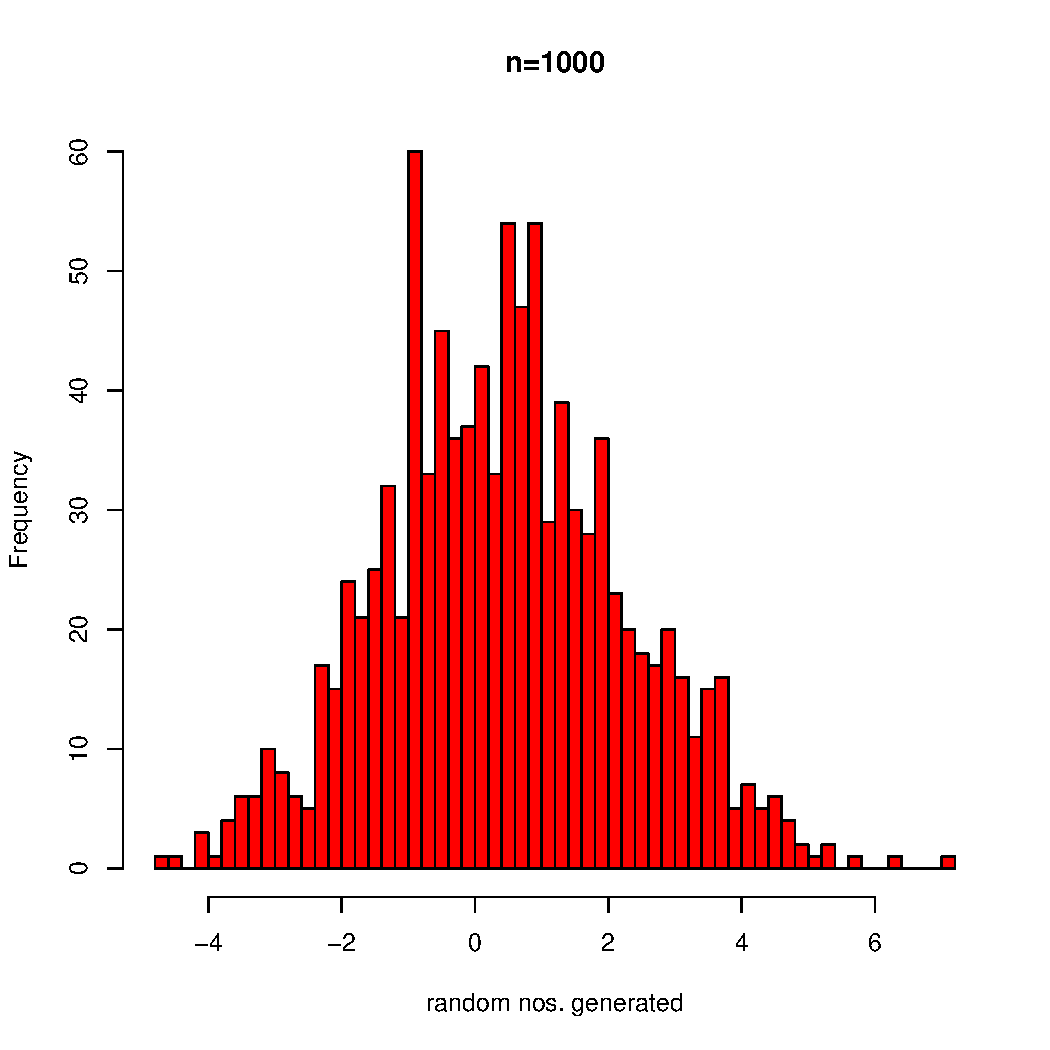
\includegraphics[scale=0.85]{Q1(1).pdf}\\\\
\\
\textbf{mean} = 0.4240377\\
\textbf{variance} = 3.805862\\
\newpage
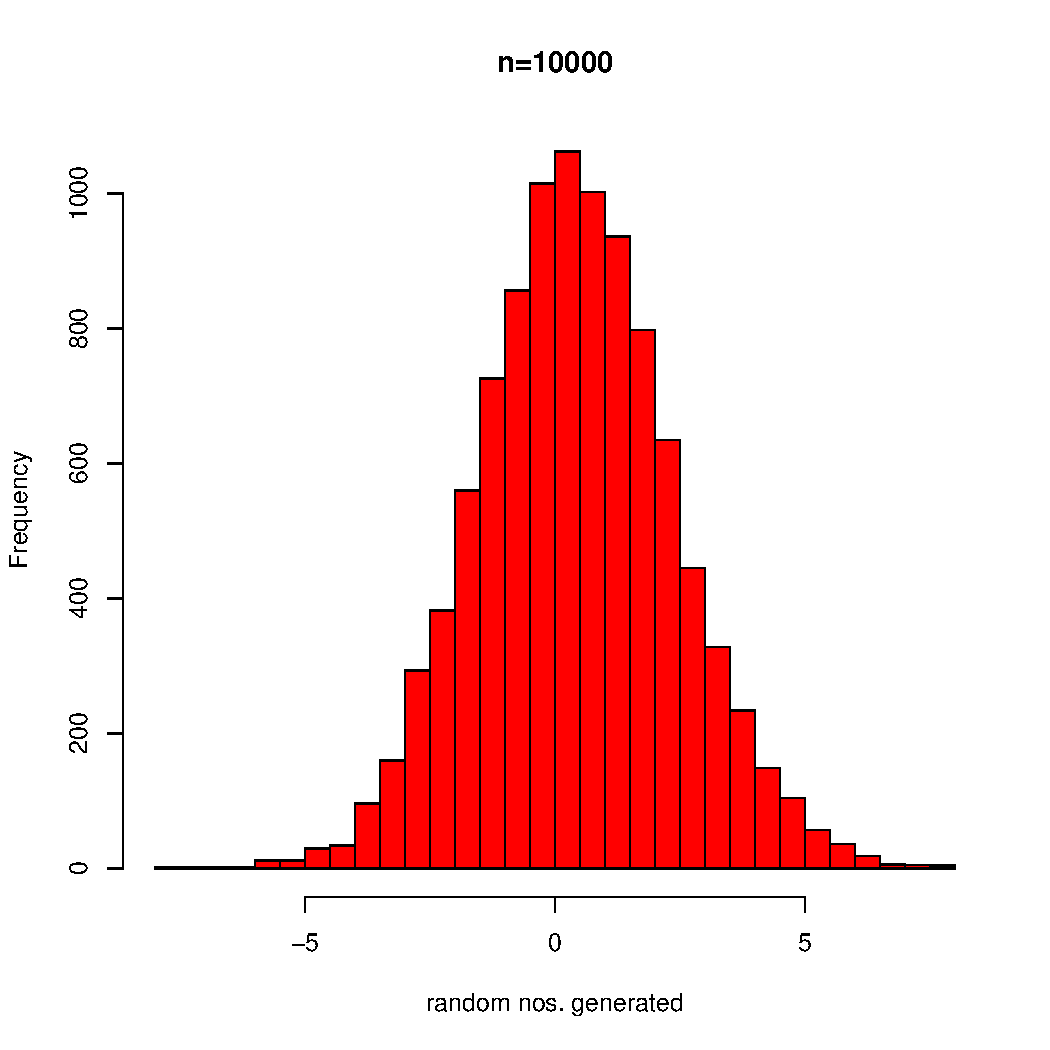
\includegraphics[scale=0.85]{Q1(2).pdf}\\\\
\\
\textbf{mean}=0.4240377\\
\textbf{variance}=3.805862\\
\newpage
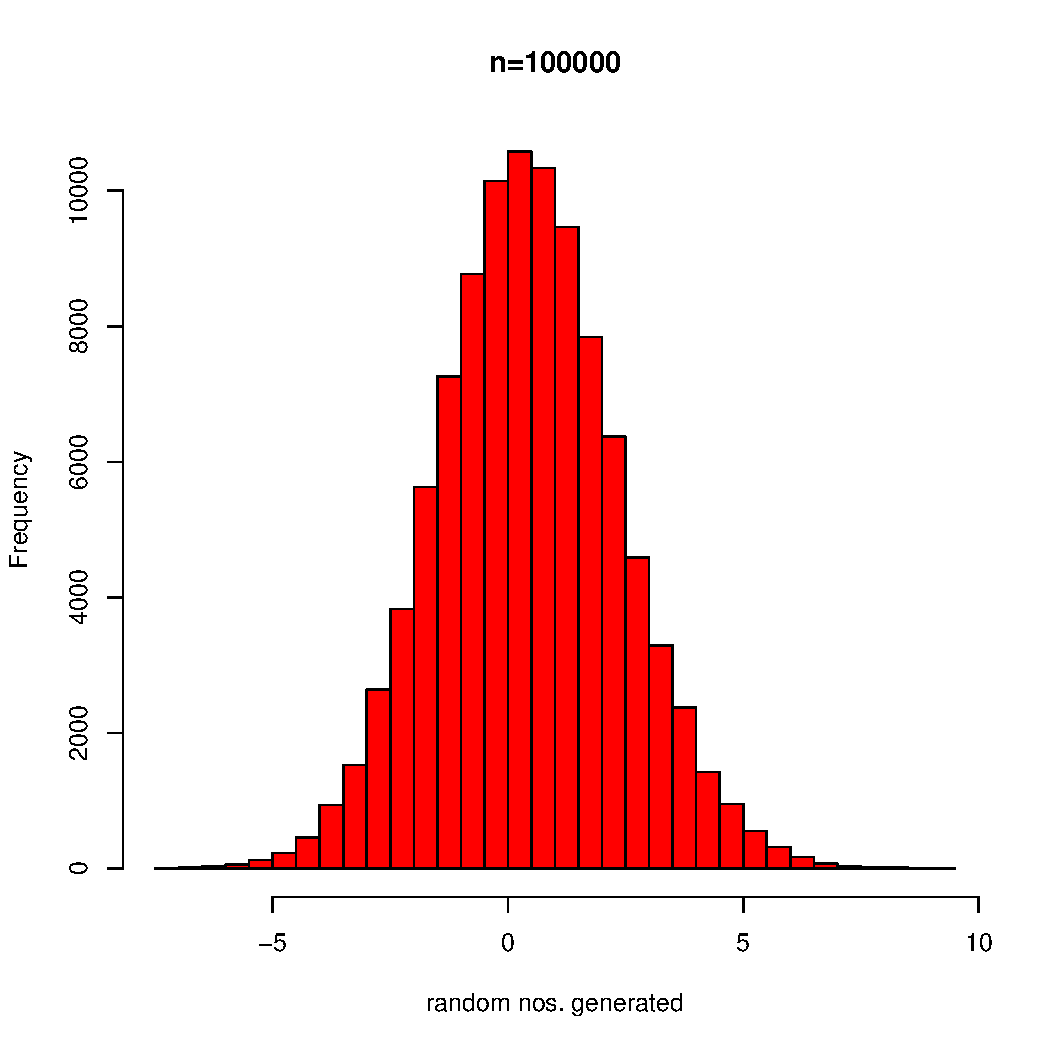
\includegraphics[scale=0.85]{Q1(3).pdf}\\\\
\\
\textbf{mean}=0.4322516\\
\textbf{variance}=3.685975\\
\newpage
\textbf{Q1(b)}\\\\\\
$F(x)=(1+\lambda)F_{1}(x)-\lambda F_{1}^2(x)$\\\\Since, PDF of a distribution is obtained by differentiating its CDF.\\\\Differentiating the above equation, we get :$$f(x)=(1+\lambda)f_1(x)-2\lambda F_1(x)f_1(x)$$\\Choosing $g(x)=f_1(x)$$$f(x)/g(x)=(1+\lambda)-2\lambda F_1(x)$$\\\\
\textbf{Q1(b) - R Code}\\\\
\begin{lstlisting}
{
 c=2;
 l=0.1;
 y=NULL;
 n=2000;
 count=0;
	
 X=rnorm(n,mean=1,sd=2);
 U=runif(n);
 P=ecdf(X);
 k=NULL;
	
 for(i in 1:n)
    {
     k[i]=((1+l)-2*l*P(X[i]))/c;
	
     if(U[i]<=k[i])
       {
	y[count]=X[i];
	count=count+1;
       }
    }
	
 print(y);
 print(count);
 hist(y, col="red",breaks=50, xlab="random nos. generated")
 print(mean(y));
 print(var(y));
}
\end{lstlisting}
\newpage
\textbf{Q1(b) - Output}\\\\\\
\textbf{\textit{Histograms :}}\\\\
For l = 0.1\\
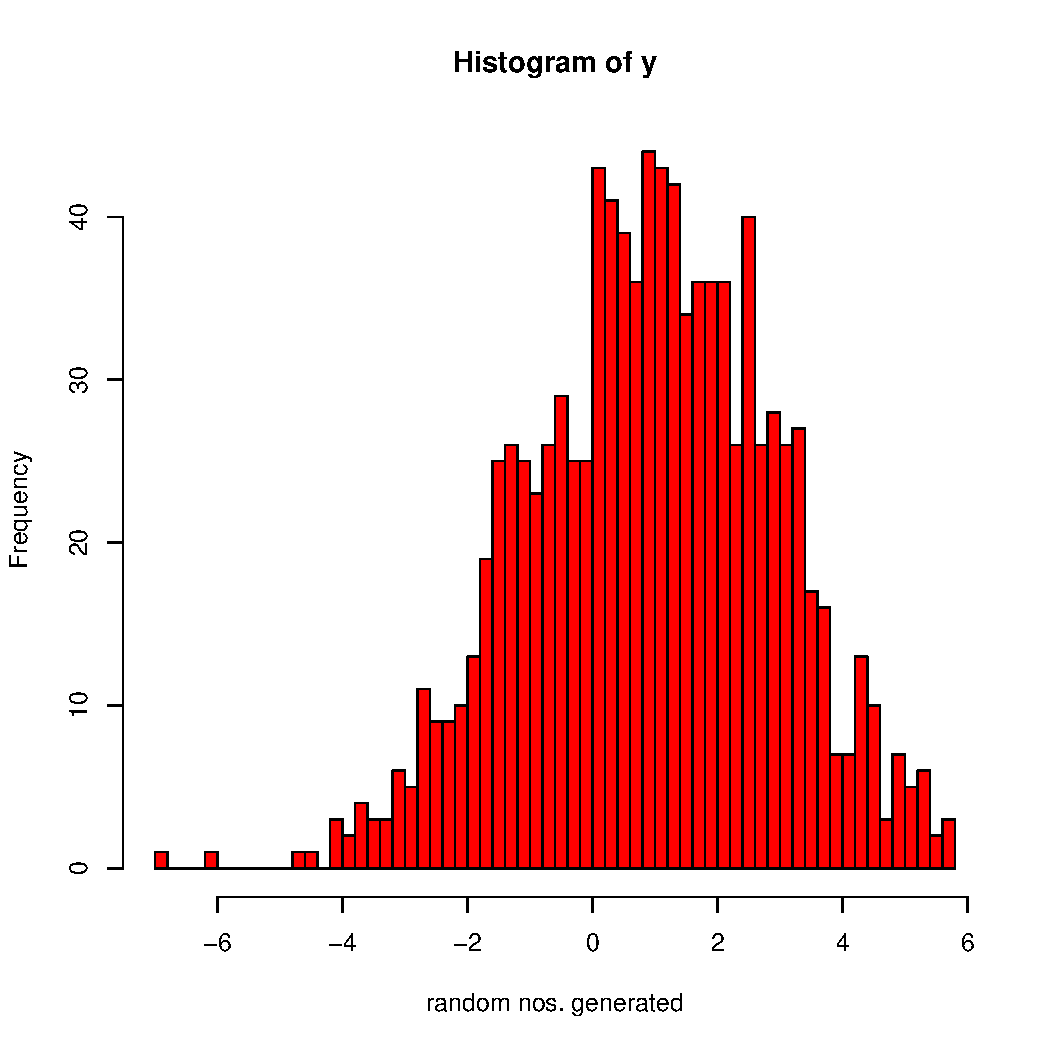
\includegraphics[scale=0.85]{Q1(4).pdf}\\
\\
\textbf{mean} = 0.4240377\\
\textbf{variance} = 3.805862\\
\newpage
For l = 0.5\\
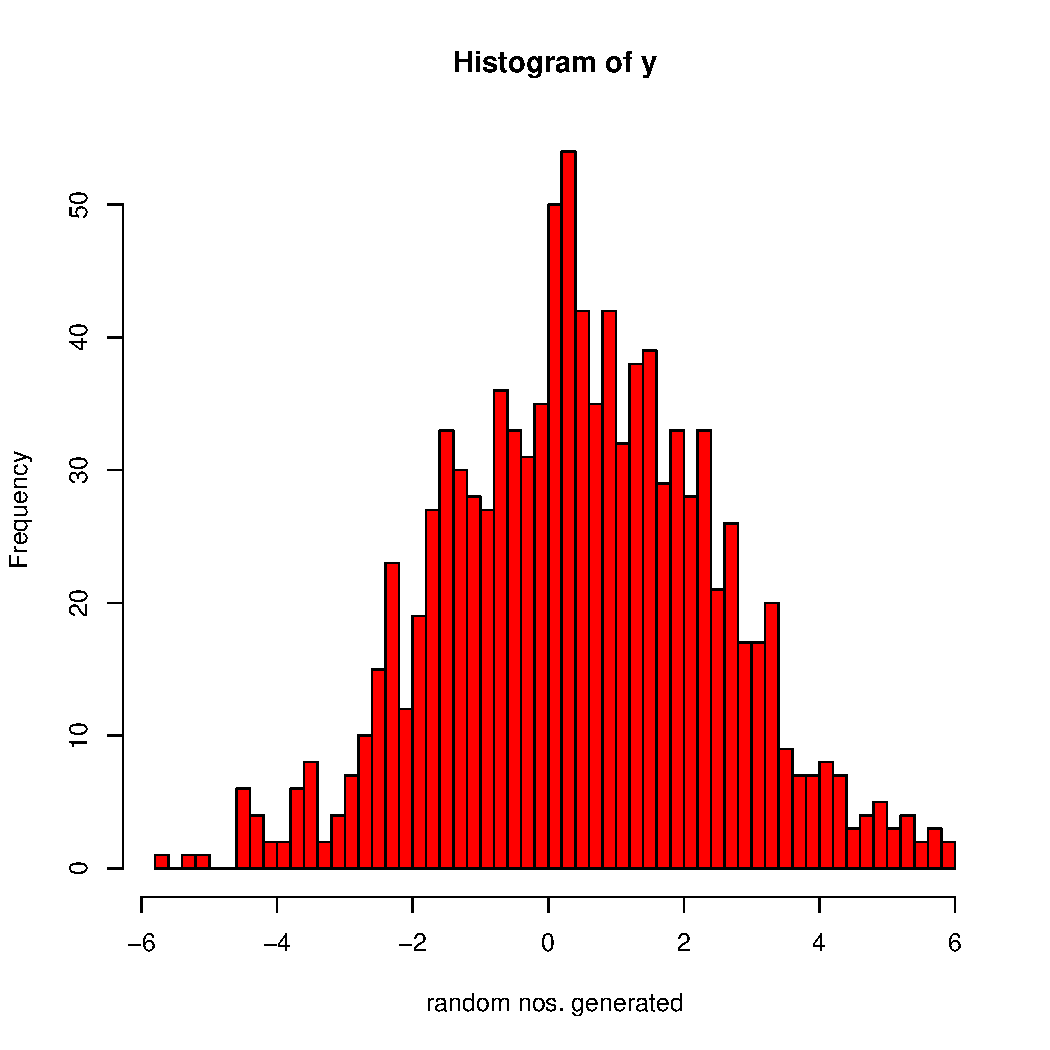
\includegraphics[scale=0.85]{Q1(5).pdf}\\\\
\\
\textbf{mean}=0.4240377\\
\textbf{variance}=3.805862\\
\newpage
For l = 0.9\\
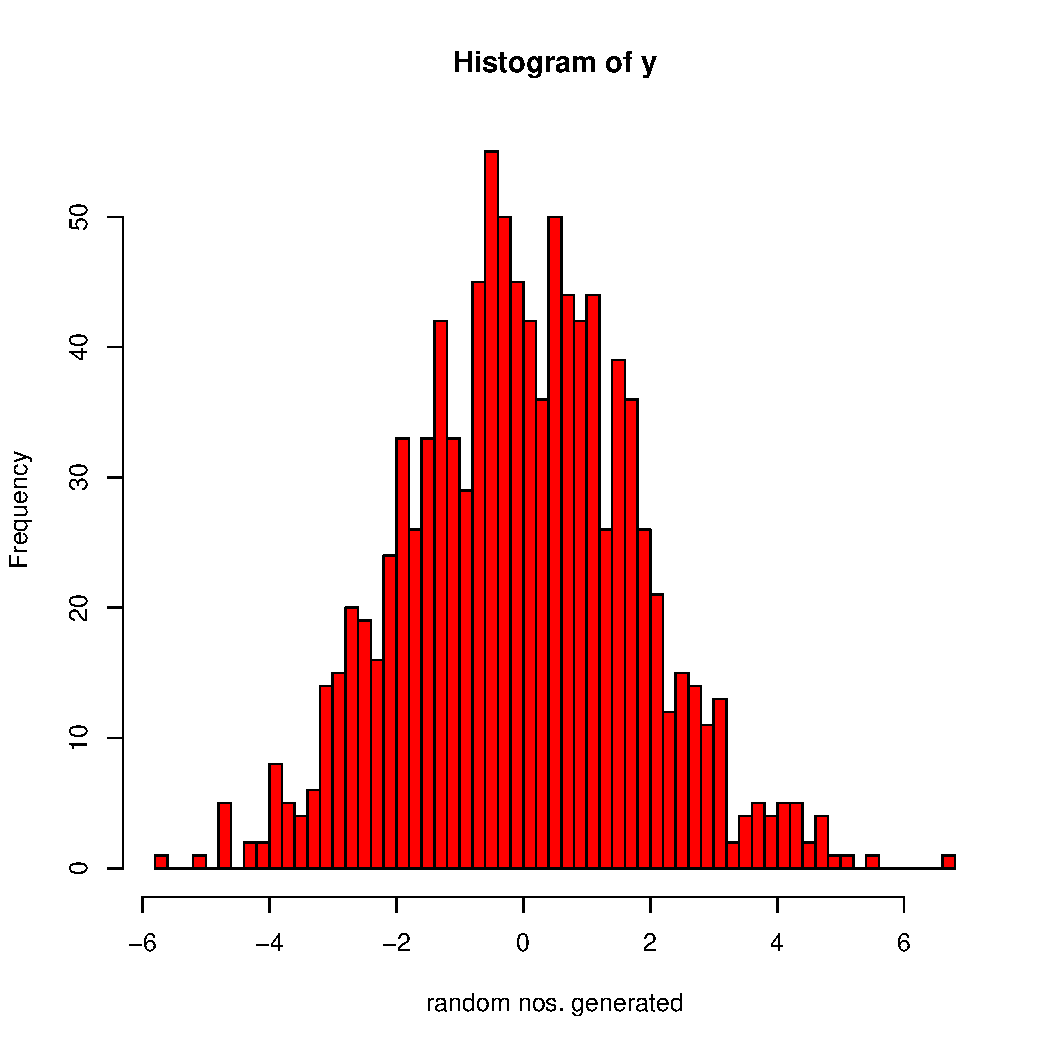
\includegraphics[scale=0.85]{Q1(6).pdf}\\\\
\\
\textbf{mean}=0.4322516\\
\textbf{variance}=3.685975\\
\end{document}
